\section{Predecessors}

\begin{frame}{VLab}
    \begin{columns}[t]
        \begin{column}{0.4\textwidth}
            \begin{itemize}
                \item The Virtual Laboratory for Earth and Planetary Materials (VLab), was
                      funded by the NSF in 2004 at the Minnesota Supercomputing Institute.
                \item VLab is a cyberinfrastructure consisting a fully integrated web
                      portal, web services, and databases for ab initio calculations of
                      planetary materials.
            \end{itemize}
        \end{column}

        \begin{column}{0.6\textwidth}
            \begin{tikzpicture}[baseline=(current bounding box.north)]
                \draw (0, 0) node {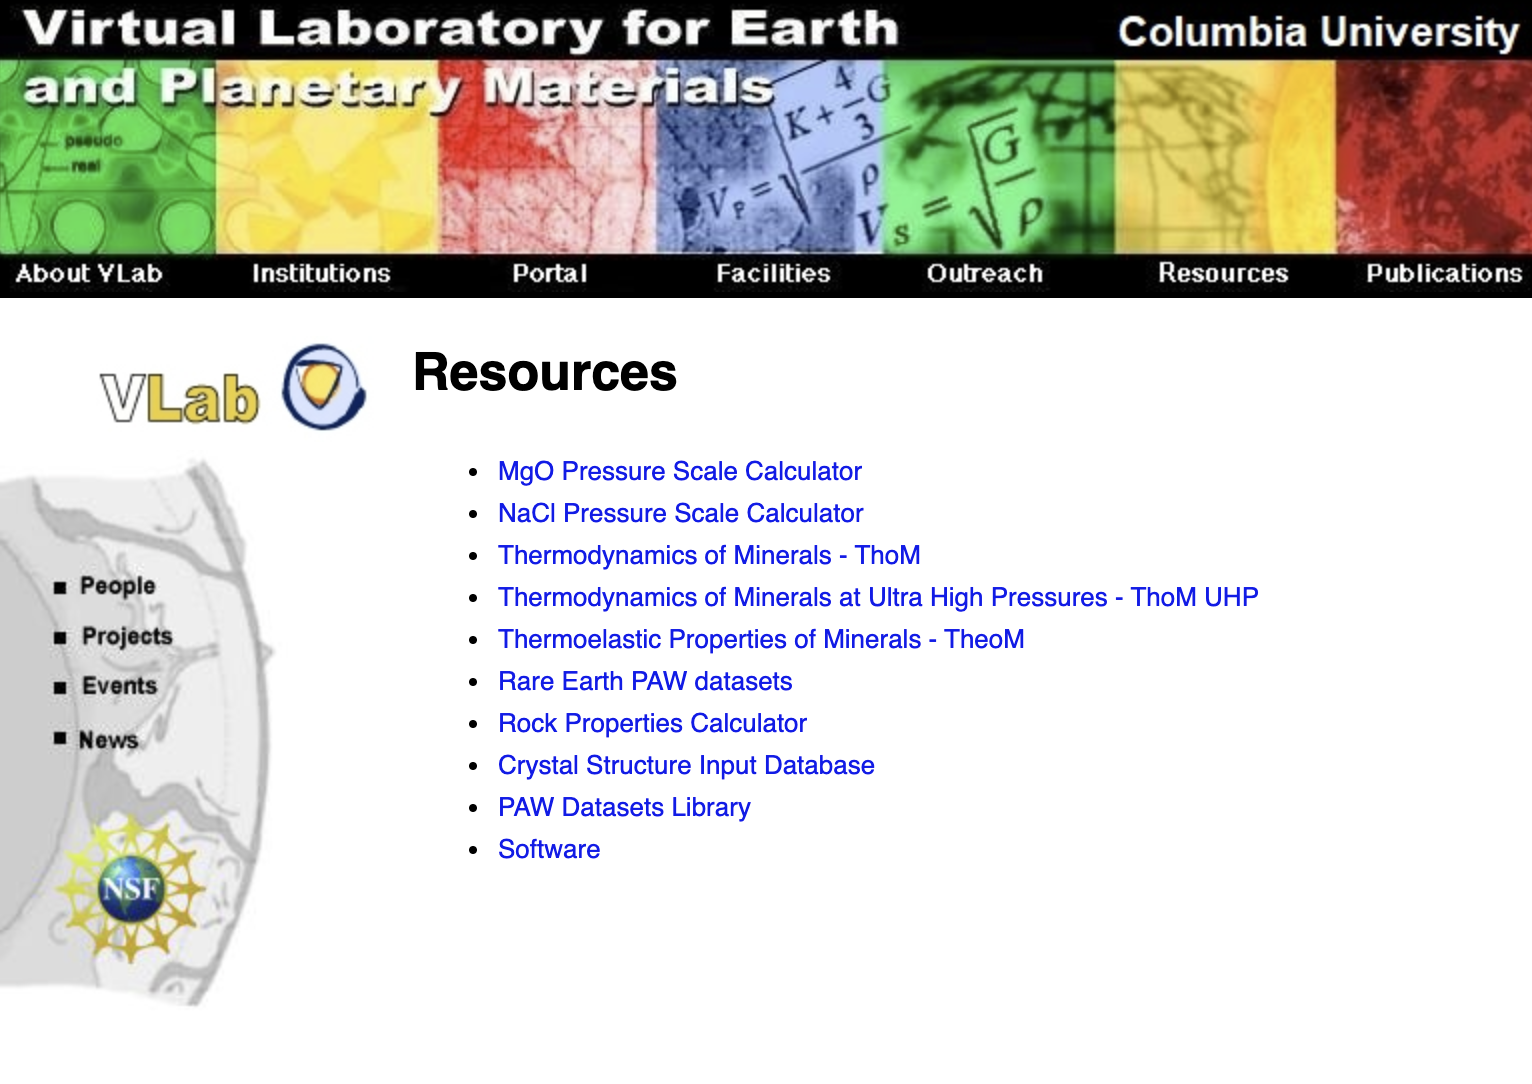
\includegraphics[width=\textwidth]{vlab}};
                \draw (1, 1) node {Hello world};
            \end{tikzpicture}
        \end{column}
    \end{columns}
    \footcitetext{DASILVA2007321}

    \begin{tikzpicture}[overlay, remember picture]
        \node[xshift=-1cm,yshift=-1cm] at (current page.north east) {\qrcode[height=2cm]{http://mineralscloud.com/resources/}};
    \end{tikzpicture}
\end{frame}
